%% ============================================================
%%  Série Avaliação na Prática — FGV CLEAR
%%  Introdução à Inferência Causal
%% ============================================================

% !TEX program = pdflatex
% !TEX encoding = UTF-8 Unicode

\PassOptionsToPackage{dvipsnames}{xcolor}
\documentclass[12pt, a4paper, openany]{book}

%% ── Codificação e Idioma ────────────────────────────────────
\usepackage[utf8]{inputenc}
\usepackage[T1]{fontenc}
\usepackage[brazil]{babel}

%% ── Fonte ───────────────────────────────────────────────────
\usepackage{tgpagella}

%% ── Matemática ──────────────────────────────────────────────
\usepackage{amsmath, amssymb, amsfonts, dsfont, amsthm}

%% ── Figuras e Tabelas ───────────────────────────────────────
\usepackage{graphicx, float}
\usepackage[labelfont=bf, font=small, justification=justified]{caption}
\usepackage{subcaption}
\usepackage{booktabs, multirow, multicol, array}
\usepackage{longtable}
\usepackage{tabularx}

%% ── Layout ──────────────────────────────────────────────────
\usepackage{geometry}
\geometry{a4paper, left=2.5cm, right=2.5cm, top=2.5cm, bottom=2.5cm}
\usepackage{setspace}
\onehalfspacing
\usepackage{fancyhdr}
\usepackage{emptypage}
\usepackage{enumitem}

%% ── TikZ e PGF ──────────────────────────────────────────────
\usepackage{csquotes}
\usepackage{tikz}
\usepackage{pgfplots}
\pgfplotsset{compat=1.18}
\usetikzlibrary{arrows.meta, positioning, decorations.pathreplacing}

%% ── Cores (paleta CLEAR) ────────────────────────────────────
\usepackage{xcolor}
\definecolor{clearblue}{HTML}{1B3A6E}
\definecolor{clearlightblue}{HTML}{5CA4A9}
\definecolor{cleardarkblue}{HTML}{003F72}
\definecolor{cleargray}{HTML}{6E6E6E}
\definecolor{salmonbg}{RGB}{252,235,230}
\definecolor{salmonframe}{RGB}{230,160,140}
\definecolor{bluebg}{RGB}{235,245,251}
\definecolor{blueframe}{RGB}{58,125,181}
\definecolor{orangebg}{RGB}{254,245,231}
\definecolor{orangeframe}{RGB}{230,126,34}
\definecolor{redbg}{RGB}{250,230,225}
\definecolor{redframe}{RGB}{180,40,40}
\definecolor{codebg}{RGB}{248,248,248}
\definecolor{codeframe}{RGB}{200,200,200}
\definecolor{codegray}{rgb}{0.45,0.45,0.45}
\definecolor{redbg}{RGB}{250,230,225}
\definecolor{redframe}{RGB}{180,40,40}
\definecolor{greenbg}{RGB}{225,242,225}
\definecolor{greenframe}{RGB}{60,140,80}

%% ── Hyperlinks e Bibliografia ───────────────────────────────
\usepackage{hyperref}
\hypersetup{
  colorlinks = true,
  linkcolor  = clearlightblue,
  urlcolor   = clearlightblue,
  citecolor  = clearlightblue,
  pdftitle   = {Guia de Cálculo de Poder},
  pdfauthor  = {FGV CLEAR}
}
\usepackage{natbib}
\bibliographystyle{plainnat}

%% ── TColorbox ───────────────────────────────────────────────
\usepackage[many]{tcolorbox}
\tcbuselibrary{breakable, skins}

%% ── Código ──────────────────────────────────────────────────
\usepackage{listings}

%% ── Cabeçalhos e Rodapés ────────────────────────────────────
\pagestyle{fancy}
\fancyhf{}
\fancyhead[R]{\small\color{clearblue}\textit{Guia CLEAR $|$ C\'alculo de Poder}}
\fancyfoot[C]{\thepage}
\renewcommand{\headrulewidth}{0.4pt}
\renewcommand{\headrule}{\hbox to\headwidth{\color{clearblue}\leaders\hrule height \headrulewidth\hfill}}

%% ── Títulos de Seção ────────────────────────────────────────
\usepackage{titlesec}
\titleformat{\chapter}[display]
  {\normalfont\huge\bfseries\color{clearblue}}
  {\chaptertitlename\ \thechapter}{20pt}{\Huge}
\titleformat{\section}
  {\normalfont\Large\bfseries\color{clearblue}}{\thesection}{1em}{}
\titleformat{\subsection}
  {\normalfont\large\bfseries\color{cleardarkblue}}{\thesubsection}{1em}{}
\titleformat{\subsubsection}
  {\normalfont\normalsize\bfseries\color{cleardarkblue}}{\thesubsubsection}{1em}{}

%% ── Numeração ───────────────────────────────────────────────
\numberwithin{equation}{chapter}
\numberwithin{table}{chapter}
\numberwithin{figure}{chapter}

%% ── Caixas Temáticas ────────────────────────────────────────
\newtcolorbox{destaquebox}[1][Destaque]{
  enhanced, breakable,
  colback=salmonbg, colframe=salmonframe, coltitle=black, fonttitle=\bfseries,
  title=#1, boxrule=0.5pt, arc=2pt,
  left=6pt, right=6pt, top=4pt, bottom=4pt
}
\newtcolorbox{notabox}[1][Nota]{
  enhanced, breakable,
  colback=bluebg, colframe=blueframe, coltitle=white, fonttitle=\bfseries,
  title=#1, boxrule=0.5pt, arc=2pt,
  left=6pt, right=6pt, top=4pt, bottom=4pt
}
\newtcolorbox{conexaobox}[1][Conex\~ao com a s\'erie]{
  enhanced, breakable,
  colback=orangebg, colframe=orangeframe, coltitle=black, fonttitle=\bfseries,
  title=#1, boxrule=0.5pt, arc=2pt,
  left=6pt, right=6pt, top=4pt, bottom=4pt
}
\newtcolorbox{exemplobox}[1][Exemplo]{
  enhanced, breakable,
  colback=greenbg, colframe=greenframe, coltitle=white, fonttitle=\bfseries,
  title=#1, boxrule=0.5pt, arc=2pt,
  left=6pt, right=6pt, top=4pt, bottom=4pt
}
\newtcolorbox{hipotesebox}[1][Hip\'otese]{
  enhanced, breakable,
  colback=salmonbg, colframe=salmonframe, coltitle=black, fonttitle=\bfseries,
  title=#1, boxrule=0.5pt, arc=2pt,
  left=6pt, right=6pt, top=4pt, bottom=4pt
}
\newtcolorbox{atencaobox}[1][Aten\c{c}\~ao]{
  enhanced, breakable,
  colback=redbg, colframe=redframe, coltitle=white, fonttitle=\bfseries,
  title=#1, boxrule=0.5pt, arc=2pt,
  left=6pt, right=6pt, top=4pt, bottom=4pt
}

%% ── Estilo de Listings ──────────────────────────────────────
\lstdefinestyle{Rstyle}{
  language         = R,
  commentstyle     = \color{codegray}\itshape,
  keywordstyle     = \color{clearblue}\bfseries,
  numberstyle      = \tiny\color{codegray},
  stringstyle      = \color{clearlightblue},
  basicstyle       = \ttfamily\small,
  breakatwhitespace= false,
  breaklines       = true,
  captionpos       = b,
  keepspaces       = true,
  numbers          = left,
  numbersep        = 8pt,
  showspaces       = false,
  showstringspaces = false,
  showtabs         = false,
  tabsize          = 2,
  frame            = single,
  rulecolor        = \color{codeframe},
  backgroundcolor  = \color{codebg},
  inputencoding    = utf8,
  extendedchars    = true,
  literate =
    {á}{{\'{a}}}1 {à}{{\`{a}}}1 {â}{{\^{a}}}1 {ã}{{\~{a}}}1
    {é}{{\'{e}}}1 {ê}{{\^{e}}}1
    {í}{{\'{i}}}1
    {ó}{{\'{o}}}1 {ô}{{\^{o}}}1 {õ}{{\~{o}}}1
    {ú}{{\'{u}}}1
    {ç}{{\c{c}}}1
    {Á}{{\'{A}}}1 {Â}{{\^{A}}}1 {Ã}{{\~{A}}}1
    {É}{{\'{E}}}1 {Ê}{{\^{E}}}1
    {Í}{{\'{I}}}1
    {Ó}{{\'{O}}}1 {Ô}{{\^{O}}}1 {Õ}{{\~{O}}}1
    {Ú}{{\'{U}}}1
    {Ç}{{\c{C}}}1
}
\lstset{style=Rstyle}

%% ── Teoremas ────────────────────────────────────────────────
\newtheorem{definition}{Defini\c{c}\~ao}[chapter]
\newtheorem{proposition}{Proposi\c{c}\~ao}[chapter]
\newtheorem{remark}{Observa\c{c}\~ao}[chapter]

%% ── Atalhos Matemáticos ─────────────────────────────────────
\newcommand{\E}{\mathbb{E}}
\newcommand{\Var}{\mathrm{Var}}
\newcommand{\Cov}{\mathrm{Cov}}
\newcommand{\indep}{\perp\!\!\!\perp}
\newcommand{\iid}{\overset{\text{i.i.d.}}{\sim}}

%% ── Metadados de Figuras/Quadros ────────────────────────────
\newcommand{\figmeta}[3]{%
  \par\vspace{4pt}%
  \begin{minipage}{\linewidth}%
  \footnotesize%
  \textbf{Fonte:} #1%
  \ifx&#2&\else\\\textbf{Elabora\c{c}\~ao:} #2\fi%
  \ifx&#3&\else\\\textbf{Nota:} #3\fi%
  \end{minipage}%
  \vspace{6pt}%
}

%% ── Profundidade de numera\c{c}\~ao ─────────────────────────
\setcounter{secnumdepth}{2}
\setcounter{tocdepth}{2}



% ============================================================
%  Compatibilidade — definições próprias do Guia de Cálculo de Poder
%  (caixa boxH e estilo de código harmonizados à paleta CLEAR)
% ============================================================

%% ── Pacotes adicionais usados no corpo ──────────────────────
\usepackage{makecell}
\usepackage{eurosym}

%% ── Cores auxiliares ────────────────────────────────────────
\definecolor{main}{HTML}{1B3A6E}   % harmonizado com clearblue
\definecolor{sub}{RGB}{235,245,251} % harmonizado com bluebg
\definecolor{codegreen}{rgb}{0,0.6,0}
\definecolor{codepurple}{rgb}{0.58,0,0.82}
\definecolor{backcolour}{rgb}{0.95,0.95,0.92}

%% ── Atalhos do corpo ────────────────────────────────────────
\providecommand{\red}[1]{{\color{red} #1}}
\providecommand{\blue}[1]{{\color{blue} #1}}
\providecommand{\ImageWidth}{11cm}
\newcolumntype{L}[1]{>{\raggedright\let\newline\\\arraybackslash\hspace{0pt}}m{#1}}
\newcolumntype{C}[1]{>{\centering\let\newline\\\arraybackslash\hspace{0pt}}m{#1}}
\newcolumntype{R}[1]{>{\raggedleft\let\newline\\\arraybackslash\hspace{0pt}}m{#1}}

%% ── Caixa de destaque (paleta CLEAR) — antes: boxH ──────────
\newtcolorbox{boxH}{
  enhanced, breakable,
  colback=bluebg, colframe=clearblue,
  boxrule=0pt, leftrule=6pt, arc=2pt,
  left=6pt, right=6pt, top=4pt, bottom=4pt
}

%% ── Estilo de código R (paleta CLEAR) ───────────────────────
\lstdefinestyle{mystyle}{
  language         = R,
  commentstyle     = \color{codegray}\itshape,
  keywordstyle     = \color{clearblue}\bfseries,
  numberstyle      = \tiny\color{codegray},
  stringstyle      = \color{clearlightblue},
  basicstyle       = \ttfamily\footnotesize,
  breakatwhitespace= false,
  breaklines       = true,
  captionpos       = b,
  keepspaces       = true,
  numbers          = none,
  numbersep        = 5pt,
  showspaces       = false,
  showstringspaces = false,
  showtabs         = false,
  tabsize          = 2,
  inputencoding    = utf8,
  extendedchars    = true,
  literate =
    {á}{{\'{a}}}1 {à}{{\`{a}}}1 {â}{{\^{a}}}1 {ã}{{\~{a}}}1
    {é}{{\'{e}}}1 {ê}{{\^{e}}}1
    {í}{{\'{i}}}1
    {ó}{{\'{o}}}1 {ô}{{\^{o}}}1 {õ}{{\~{o}}}1
    {ú}{{\'{u}}}1
    {ç}{{\c{c}}}1
    {Á}{{\'{A}}}1 {Â}{{\^{A}}}1 {Ã}{{\~{A}}}1
    {É}{{\'{E}}}1 {Ê}{{\^{E}}}1
    {Í}{{\'{I}}}1
    {Ó}{{\'{O}}}1 {Ô}{{\^{O}}}1 {Õ}{{\~{O}}}1
    {Ú}{{\'{U}}}1
    {Ç}{{\c{C}}}1
}
\lstset{style=mystyle}

\begin{document}

\frontmatter

% ============================================================
% CAPA
% ============================================================
\thispagestyle{empty}
\begin{center}
\vspace*{3cm}

{\Large\bfseries\color{clearlightblue} S\'ERIE: AVALIA\c{C}\~AO NA PR\'ATICA}

\vspace{1.8cm}

{\Huge\bfseries\color{clearblue} C\'alculo de Poder }

\vspace{2.2cm}

{\large FGV CLEAR $|$ FGV EESP}

\vspace{0.5cm}

{\large Maio de 2026}

\vfill
\end{center}
\newpage

% ============================================================
% FICHA TÉCNICA
% ============================================================
\thispagestyle{empty}
\vspace*{1.5cm}

{\Large\bfseries\color{clearblue} Ficha T\'ecnica}

\bigskip

\noindent\textbf{Equipe t\'ecnica:} FGV CLEAR.

\bigskip

\noindent\textbf{Apresenta\c{c}\~ao.} Este guia integra a s\'erie de publica\c{c}\~oes \textit{Avalia\c{c}\~ao na Pr\'atica}, desenvolvida pelo FGV CLEAR com o objetivo de ampliar o acesso a conhecimentos sobre monitoramento e avalia\c{c}\~ao com foco em pol\'iticas p\'ublicas.

\medskip

\noindent Fundado em 2015, o FGV CLEAR tem se dedicado ao fortalecimento da cultura de gest\~ao orientada por evid\^encias no Brasil e em pa\'ises lus\'ofonos. Com sede na Escola de Economia de S\~ao Paulo da Funda\c{c}\~ao Getulio Vargas (FGV EESP), o FGV CLEAR atua como centro regional da Iniciativa CLEAR (\textit{Centers for Learning on Evaluation and Results}).

\medskip

\noindent Saiba mais sobre o FGV CLEAR e acesse outras publica\c{c}\~oes em: \textbf{www.fgvclear.org}

\vfill

\noindent{\small\color{cleargray}%
\textbf{Cita\c{c}\~ao recomendada:} FGV CLEAR. (\the\year). \textit{Guia de C\'alculo de Poder}. S\'erie Avalia\c{c}\~ao na Pr\'atica. S\~ao Paulo: FGV CLEAR.

\medskip

\noindent Os textos desta publica\c{c}\~ao s\~ao de responsabilidade exclusiva dos autores. As opini\~oes expressas n\~ao refletem necessariamente a posi\c{c}\~ao das institui\c{c}\~oes parceiras.}

\newpage

% ============================================================
% SOBRE ESTE GUIA
% ============================================================
\thispagestyle{empty}
\section*{Sobre este guia}
Antes de rodar um experimento, vale fazer uma pergunta incomoda: e se ele n\~ao
detectar nada? Um ensaio aleatorizado bem desenhado pode terminar sem efeito
estat\'isticamente significante n\~ao porque a pol\'itica n\~ao funciona, mas porque
a amostra era pequena demais para enxergar um efeito que existe. Calcular poder
\'e o exerc\'icio que separa essas duas situa\c{c}\~oes antes de gastar tempo e or\c{c}amento
em campo.

O conceito central \'e o efeito m\'inimo detect\'avel, ou MDE --- o menor efeito
verdadeiro que o experimento tem chance razo\'avel de identificar, dado o tamanho
da amostra, a vari\^ancia do desfecho e o n\'ivel de signific\^ancia. Pensar em
termos de MDE inverte a l\'ogica usual: em vez de perguntar qual o efeito
estimado, pergunta-se qual efeito o desenho seria capaz de detectar caso
estivesse l\'a. Um experimento cujo MDE \'e maior do que qualquer efeito
plaus\'ivel da interven\c{c}\~ao nasce condenado a um resultado nulo pouco informativo.

O guia parte do c\'alculo de poder no caso mais simples e vai relaxando hip\'oteses
conforme os desenhos reais exigem. Trata da convers\~ao entre poder e tamanho de
amostra, do problema de cumprimento imperfeito --- quando nem todos os designados
ao tratamento de fato o recebem ---, dos experimentos aleatorizados por grupo,
em que a unidade de aleatoriza\c{c}\~ao n\~ao \'e o indiv\'iduo, da estratifica\c{c}\~ao como
ferramenta para ganhar precis\~ao e do ajuste para m\'ultiplas hip\'oteses. Cada
t\'opico combina a deriva\c{c}\~ao da f\'ormula com simula\c{c}\~oes em R que reproduzem o
c\'alculo.

O leitor que conhece o \textit{Guia CLEAR de Introdu\c{c}\~ao \`a Infer\^encia Causal}
reconhecer\'a que poder \'e a contraparte de planejamento da etapa de infer\^encia:
enquanto a infer\^encia quantifica a incerteza depois de observar os dados, o
c\'alculo de poder antecipa, antes da coleta, quanta incerteza o desenho vai
deixar. Os dois lados precisam conversar para que um experimento valha o que
custa.
\newpage

% ============================================================
% COMO LER ESTE GUIA
% ============================================================
\thispagestyle{empty}
\section*{Como ler este guia}
O guia alterna a deriva\c{c}\~ao das f\'ormulas com sua implementa\c{c}\~ao pr\'atica.
Dois elementos se repetem ao longo dos cap\'itulos e merecem aten\c{c}\~ao.

\vspace{0.2cm}
\begin{boxH}
\textbf{Caixa de destaque.} A barra azul \`a esquerda marca os pontos em que uma
escolha de desenho --- tamanho de amostra, n\'ivel de agrupamento, regra de
ajuste --- altera diretamente o poder do experimento. \'E onde a teoria do
cap\'itulo vira decis\~ao pr\'atica.
\end{boxH}
\vspace{0.3cm}

\noindent O \textbf{c\'odigo em R} aparece em blocos monoespa\c{c}ados, prontos para
reprodu\c{c}\~ao, logo ap\'os a f\'ormula correspondente. As subse\c{c}\~oes intituladas
``Praticando'' levam o leitor da f\'ormula anal\'itica \`a simula\c{c}\~ao, mostrando
que os dois caminhos chegam ao mesmo n\'umero.

\vspace{0.3cm}
\noindent O guia faz refer\^encia ao \textit{Guia CLEAR de Monitoramento e
Avalia\c{c}\~ao de Pol\'iticas P\'ublicas: do diagn\'ostico \`a decis\~ao} ---
doravante \textbf{Guia CLEAR de M\&A} --- para o ciclo da pol\'itica p\'ublica, e ao
\textit{Guia CLEAR de Introdu\c{c}\~ao \`a Infer\^encia Causal} para o arcabou\c{c}o de
identifica\c{c}\~ao, estima\c{c}\~ao e infer\^encia.
\newpage

\tableofcontents
\newpage

% ============================================================
% CONTEÚDO
% ============================================================

\mainmatter

\chapter{Introdução}\label{introducao}

\input{Sections/sec1_introducao}

\chapter{Cálculo de Poder}\label{poder}

\input{Sections/sec2_calculo_de_poder}

\chapter{Imperfect Compliance}\label{late}

\input{Sections/sec3_imperfect_compliance}

\chapter{RCT Agrupado}\label{cluster}

\input{Sections/sec4_clustered_rct}

\chapter{Estratificação}\label{strat}

Muitas vezes, a aleatorização é realizada em blocos, um método amplamente utilizado para garantir maior controle sobre o balanceamento das covariadas pré-tratamento entre os grupos de tratamento e controle. Essa abordagem, também conhecida como estratificação, é especialmente útil quando desejamos assegurar que certos fatores importantes sejam equilibrados antes da aplicação do tratamento, como idade, gênero ou características socioeconômicas. Além de promover um balanceamento mais preciso, a aleatorização em blocos tende a reduzir a variância do estimador de interesse, o que resulta em ganhos significativos de eficiência na análise. Essa característica torna os desenhos estratificados particularmente atrativos em contextos onde a precisão das estimativas é crucial, maximizando o poder estatístico do experimento sem aumentar o tamanho da amostra.

No nosso exemplo empírico, imagine que estamos interessados em garantir balanceamento para algumas variáveis demográficas que temos disponíveis no período pré-tratamento, como gênero, raça e faixa de renda. Podemos criar grupos de alunos com essas características em comum e, dentro de cada grupo, $g$, aleatorizamos quem receberá uma vaga numa escola com ensino técnico. Podemos estimar o efeito do tratamento para cada um desses grupos como 

\begin{equation}
    \hat{\beta}_g = \Bar{Y}_{1,g} - \Bar{Y}_{0,g}
\end{equation}

\noindent em que $\Bar{Y}_{d,g}$ e a média dos alunos com status de tratamento $d \in \{0,1\}$ dentro do bloco $g$. A variância do nosso estimador para cada grupo $g$ é dada por

\begin{equation}\label{varg}
    \mathrm{Var}(\hat{\beta}_g) = \frac{\sigma^2_{1,g}}{N_{1,g}} + \frac{\sigma^2_{0,g}}{N_{0,g}}
\end{equation}

\noindent em que $\sigma^2_{d,g} = \mathrm{Var}(Y_{i,g}(d))$ e $N_{d,g}$ é o número de alunos com status de tratamento $d \in \{0,1\}$ no grupo $g$. Podemos estimar o efeito do tratamento para todos os grupos simplesmente fazendo a média de todos os estimadores por grupo e ponderando pela proporção de alunos em cada grupo, $\frac{N_g}{N}$,

\begin{equation}
    \hat{\beta} = \sum_{g=1}^G \hat{\beta}_g \frac{N_g}{N}
\end{equation}

Com isso, a variância do nosso estimador do efeito médio de tratamento é dada por

\begin{equation}\label{vartotal}
    \mathrm{Var}(\hat{\beta}) = \sum_{g=1}^G \mathrm{Var}(\hat{\beta}_g) \left(\frac{N_g}{N}\right)^2
\end{equation}

Utilizando a variância do estimador para cada grupo, dada pela equação \ref{varg}, podemos calcular o MDE para cada bloco $g$,

\begin{equation}\label{mde3}
    MDE_g = (t_{\frac{\alpha}{2}} + t_{1-\kappa})\sqrt{\frac{\sigma^2_{1,g}}{N_{1,g}} + \frac{\sigma^2_{0,g}}{N_{0,g}}}
\end{equation}

Para calcularmos o MDE do efeito de tratamento para todos os grupos, basta calcularmos a média dos MDE's de cada grupo, ponderando pela proporção de alunos em cada grupo,

\begin{equation}\label{mdeblock}
    MDE = \sum_{g=1}^G MDE_g \frac{N_g}{N}
\end{equation}

A fórmula dada pela equação \ref{mdeblock} é equivalente a derivarmos o MDE a partir da variância do estimador do efeito de tratamento para todos os grupos, dado pela equação \ref{vartotal}.

Um caso extremo da aleatorização em blocos é a \textbf{aleatorização por pares}\footnote{Matched-pairs randomization.}, isto é, os alunos são pareados de acordo com suas características em comum e, dentro de cada par, um aluno é aleatorizado para receber o tratamento, enquanto o outro é alocado para o grupo de controle. O procedimento para calcular o MDE nesse caso seria igual ao para a aleatorização em blocos. Porém, não conseguimos estimar a variância do estimador para cada um dos pares, dada pela equação \ref{varg}, já que temos apenas um aluno tratado e um aluno não tratado em cada um dos pares. Isso fará com que o teste $t$ seja conservador, isto é, a probabilidade de rejeitarmos a hipótese nula é menor do que o $\alpha$ especificado. \cite{bai2022} deriva inferência exata para este caso, propondo ajustes no teste. Em caso de aleatorização por pares, iremos focar em calcular o MDE por meio de simulações, como veremos na próxima seção.

Podemos derivar o MDE para casos de \textbf{efeitos heterogêneos} e \textbf{múltiplos tratamentos} da mesma forma que derivamos para o caso de aleatorização estratificada. No caso de efeitos heterogêneos, podemos separar nossa amostra entre os grupos dos quais gostaríamos de medir a heterogeneidade do tratamento e, para calcularmos o MDE do efeito total, basta fazer uma média ponderada dos MDE's de cada grupo. Por exemplo, se estamos interessados na heterogeneidade do efeito de estar matriculado numa escola de ensino técnico entre os diferentes níveis de renda dos alunos, basta calcularmos os MDE's separadamente para cada um desses níveis de renda. No caso de múltiplos tratamentos, calculamos o MDE separadamente para cada um desses grupos de tratamento. No nosso exemplo empírico, se tivermos dois tipos diferentes de escola de ensino técnico sendo ofertadas, podemos calcular o MDE para cada uma delas. 

\section{Praticando: Simulações}

Nesta seção, iremos calcular o MDE para o caso de experimento estratificados apenas através de simulações. Ao aleatorizarmos de forma estratificada, entendemos que as variâncias dos erros vão ser diferentes dentro de cada bloco. Portanto, utilizar a fórmula analítica seria útil para calcularmos o MDE em termos de desvio padrão para um bloco específico, mas não para o agregado.\footnote{Note que, para calcularmos o MDE pela fórmula analítica em para um grupo específico, basta repetirmos o procedimento da Seção \ref{rct_fa} com os valores adequados para o grupo em questão.}

Começamos o código pela limpeza do ambiente e, em seguida, carregamos os pacotes necessários. Novamente iremos utilizar o pacote \texttt{lfe}, agora para rodarmos regressões de efeito fixo. Ainda, escolhemos uma \textit{seed} aleatória e, por fim, carregamos a base de dados \texttt{base\_rct\_block.csv}.

\begin{boxH}
\begin{lstlisting}[language = R]
# Limpar o ambiente 
rm(list=ls())

# Carregando pacotes necessários

library(tidyverse)
library(randomizr)
library(lfe)

# Fazendo com que as simulações se tornem reproduzíveis
set.seed(42)

# Base de dados
base_rct_block <- read.csv("Base/base_rct_block.csv")
\end{lstlisting}
\end{boxH}

Para a simulação, iremos utilizar a função \texttt{block\_ra} do pacote \texttt{randomizr} para aleatorizarmos em blocos. Na base em questão, temos diversas escolas localizadas em diferentes municípios. Iremos estratificar a nível de municípios, aleatorizando 50\% das escolas de cada município para receberem o programa de ensino técnico. Como estamos estratificando a nível de município, devemos fazer uma regressão com efeito fixo de município. Novamente, clusterizamos o erro padrão a nível de escola, já que este também é um Clustered RCT. Por fim, armazenamos os erros padrões estimados de cada uma das 100 iterações e calculamos o MDE a partir da média dos erros padrões estimados.  

\begin{boxH}
\begin{lstlisting}[language = R]
# Criando vetor com 100 entradas para armazenar os erros padrões
se_block <- c(rep(NA, 100))

# Simulando 100 vezes o erro padrão
for (i in 1:100) {
  
  # aleatorizando por blocos (municípios)
  df <- base_rct_block %>%
    mutate(D = block_ra(blocks=id_mun, prob=0.5))
  
  
  reg_block <- felm(y~D|id_mun|0|id_escola,data=df) #regressão com efeito fixo de mun
  se_block[i] <- reg_block$se[1] # armazenando erro padrão
  
}

# Calculando MDE
MDE_block = 2.8*mean(se_block)
print(MDE_block)
\end{lstlisting}
\end{boxH}

\chapter{Múltiplas Hipóteses}\label{multihip}

Em muitas pesquisas, estamos interessados no efeito do tratamento em mais de uma variável. Nesses casos, é comum com que o pesquisador planeje corrigir o teste por múltiplas hipóteses. Quando estamos testando hipóteses para múltiplas variáveis diferentes, a probabilidade de rejeitarmos uma hipótese nula verdadeira para pelo menos uma das variáveis é maior do que nível de significância, $\alpha$, utilizado em cada um dos testes. Por exemplo, se testarmos 10 hipóteses independentes ao nível de significância de 5\%, então pelo menos uma hipótese nula verdadeira será rejeitada com probabilidade de 40\%.\footnote{A probabilidade de nenhuma das hipóteses nulas verdadeiras serem rejeitadas é de $(1-0.05)^{10}$. Portanto, a probabilidade de pelo menos uma hipótese nula verdadeira ser rejeitada é de $1 - (1-0.05)^{10} \approx 40\%$.}

Um jeito comum de corrigirmos por hipóteses múltiplas é separando as variáveis de interesse em diferentes famílias. A tabela \ref{primary_outcomes} é um exemplo de separação para nosso exemplo empírico. A \textbf{Família I} se refere às variáveis de mercado de trabalho, enquanto que a \textbf{Família II} se refere às variáveis de desempenho escolar. Ao agruparmos por famílias, estamos interessados em ver se o efeito do tratamento numa família de variáveis é significantemente diferente de zero (veja Anderson, 2008).


\begin{table}[h]
\centering
\caption{\sc Famílias de Variáveis de Interesse}
\label{primary_outcomes}
\resizebox{\textwidth}{!}{\begin{tabular}{lll}
\toprule
 & \textbf{Tipo} & \textbf{Variáveis} \\
 \midrule
  \multirow{2}{*}{\textbf{Família I.}} & \multirow{2}{*}{Mercado de Trabalho}   & \textbf{1.} Está empregado ou não \\
  & &\textbf{2.} Formal ou informal \\
    \midrule

  \multirow{3}{*}{\textbf{Família II.} } & \multirow{3}{*}{Desempenho Escolar} & \parbox{7cm}{\textbf{3.} Nota na prova} \\
             & &\textbf{4.} Frequência\\
             & &\textbf{5.} Está matriculado ou não\\
\bottomrule
\end{tabular}}

\end{table}

Para levarmos o teste de múltiplas hipóteses em consideração quando estamos calculando poder, podemos corrigir o nível de significância que estamos utilizando no cálculo do MDE. Um método comum e prático é ajustar o nível de significância para o tamanho de cada família, utilizando a correção de \v{S}idák:
\begin{equation}
    \alpha_h = 1 - (1-0.05)^{\frac{1}{h}}
\end{equation}

\noindent em que $h$ é o número de variáveis dentro da família que estamos querendo testar a hipótese. Note que se $h = 1$, temos o mesmo $\alpha = 0.05$. Ao aumentarmos $h$, o nível de significância que iremos utilizar diminui, fazendo com que a probabilidade de rejeitarmos pelo menos uma hipótese nula verdadeira seja de 5\%.\footnote{Isso acontece caso as hipóteses sejam independentes. Caso elas tenham correlação positiva, o teste é conservador e, caso a correlação seja negativa, o teste é inválido. Um jeito comum de evitar correlação negativa entre os teste é mudar o sinal das variáveis para que a direção positiva delas indique uma ``melhoria'' na variável (veja \citealp{anderson2008}).} Existem outros métodos que podem ser utilizados, como a correção de Bonferroni ou a correção de Holm (veja \citealp{anderson2008}), porém iremos utilizar apenas a correção de \v{S}idák nos nossos exemplos empíricos na próxima seção.

\section{Praticando: Fórmula Analítica}

Nesta seção, iremos calcular o MDE para o caso de múltiplas hipóteses apenas utilizando a fórmula analítica. Aqui, estamos levando em consideração apenas a correção do nível de significância, mas não entraremos em detalhes a respeito do teste de múltiplas hipóteses.\footnote{Existem várias maneiras de testarmos múltiplas hipóteses conjuntamente. Ao termos acesso aos dados, além de corrigirmos o nível de significância, temos que nos preocupar em como agregar as variáveis para o teste conjunto. Veja \cite{anderson2008} para mais detalhes deste assunto.}

Primeiramente, iremos limpar o ambiente de trabalho, carregar os pacotes necessários e definir os parâmetros que estarão fixos no cálculo do MDE.

\begin{boxH}
\begin{lstlisting}[language = R]
# Limpar o ambiente 
rm(list=ls())

# Carregando pacotes necessários
library(tidyverse)

# Parâmetros para cálculo analítico do MDE
t.kappa = 0.84 # poder de 80%
t.alpha = 1.96 # nível de significância de 5%
P = 0.5 # Porcentagem de tratados de 50%
\end{lstlisting}
\end{boxH}

Em seguida, iremos criar uma função para calcular o nível de significância ajustado e outra função para calcular o valor crítico do nível de significância ajustado, dependendo do número de variáveis dentro de uma família, $h$.

\begin{boxH}
\begin{lstlisting}[language = R]
# Correção de Sidák

alpha.h = function(h){1 - (1 - 0.05)^(1/h)}

# Valor crítico variando com h

t.alpha.h = function(h){qnorm(1-alpha.h(h)/2)}

\end{lstlisting}
\end{boxH}

Com a função do valor crítico ajustado, podemos criar uma função para o cálculo do MDE variando tanto o tamanho da amostra, $N$, quanto o número de hipóteses a serem testadas conjuntamente, $h$.

\begin{boxH}
\begin{lstlisting}[language = R]
# Fórmula analítica variando N e h

MDE.h = function(N,h){(t.kappa+t.alpha.h(h))*((1/(P*(1-P)))^0.5)*((1/N)^0.5)}
\end{lstlisting}
\end{boxH}

O bloco de código abaixo produz o gráfico da Figura \ref{fig:mde_h}. Nele, calculamos o MDE em termos de desvios padrões variando o tamanho da amostra de 500 a 3500. Produzimos três curvas no gráfico, variando o número de hipóteses que estão sendo testadas conjuntamente. Note que quanto mais hipóteses testamos conjuntamente, maior o tamanho do MDE.


\begin{boxH}
\begin{lstlisting}[language = R]
# Gráfico do MDE variando N, para h = {1,2,3}.

ggplot() + xlim(500, 3500) +
  geom_function(fun = MDE.h, args = list(h = 1), aes(colour = "h = 1"), linewidth = 0.8) +
  geom_function(fun = MDE.h, args = list(h = 2), aes(colour = "h = 2"), linewidth = 0.8) +
  geom_function(fun = MDE.h, args = list(h = 3), aes(colour = "h = 3"), linewidth = 0.8) +
  labs(y = "MDE", x = "N") +
  theme_classic() +
  guides(colour=guide_legend(title=""))

\end{lstlisting}
\end{boxH}

\begin{figure}[h]
    \centering
    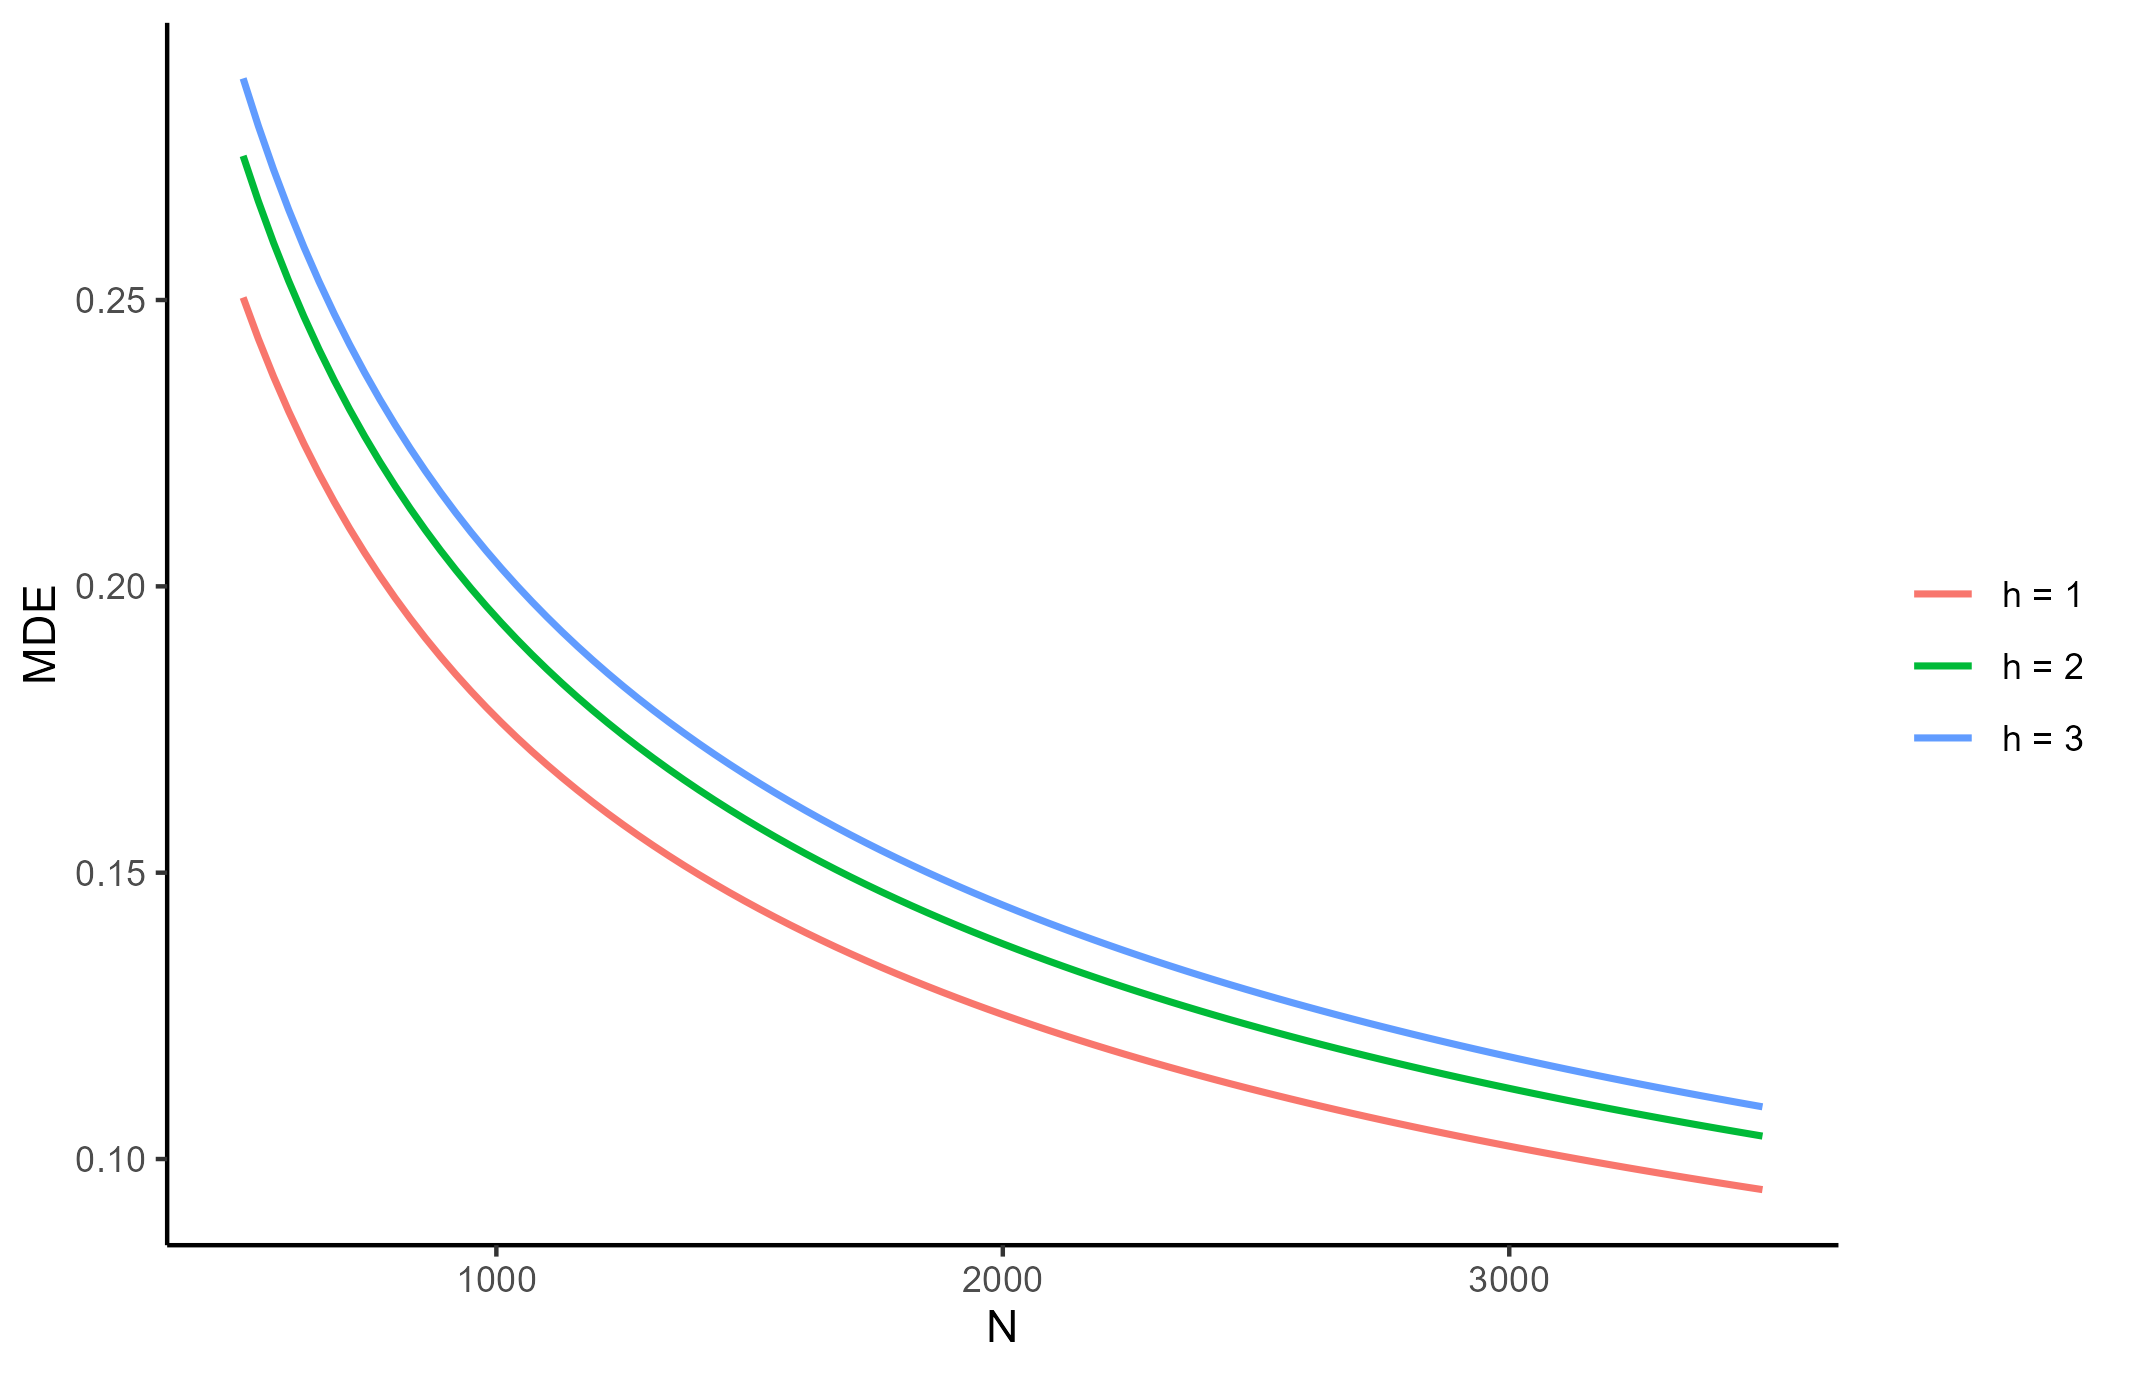
\includegraphics[width=0.8\linewidth]{Figuras/mde_h.png}
    \caption{Gráfico do MDE em termos de desvio padrão variando o tamanho da amostra de 500 a 3500 para diferentes valores de hipóteses a serem testadas conjuntamente.}
    \label{fig:mde_h}
\end{figure}

\chapter{Conclusão}\label{conclusao}

\input{Sections/sec7_conclusao}


% ============================================================
% REFERÊNCIAS
% ============================================================
\backmatter
\setlength\bibsep{0pt}
\bibliography{ref}

\end{document}
